\subsection{Policy-Based Reinforcement Learning}

Policy-Based Reinforcement Learning konzentriert sich auf das direkte Lernen einer Policy \(\pi(s)\), die Zuständen \(s\) Aktionen \(a\) zuordnet. Diese Methoden, insbesondere Policy Gradient Ansätze, sind effektiv in Umgebungen mit diskreten und kontinuierlichen Aktionsräumen.\cite{SuttonBarto2018}.

\paragraph{Mathematische Grundlagen}
Die Aktualisierung der Policy-Parameter \(\theta\) erfolgt anhand des Policy Gradient Ansatzes, wie in der folgenden Gleichung dargestellt:
\begin{equation} 
\nabla_{\theta} J(\theta) = \mathbb{E}_{\pi} \left[ \nabla_{\theta} \log \pi(a | s; \theta) \cdot R(s, a) \right]
		\label{eq:policy_gradient}
\end{equation}

Hierbei ist \(J(\theta)\) die zu maximierende Zielfunktion, \(R(s, a)\) die Belohnung und \(\theta\) die Policy-Parameter \cite{russell2021ai}. Die Aktionen werden basierend auf der Wahrscheinlichkeitsverteilung der Policy, häufig modelliert durch eine Softmax-Funktion, ausgewählt \cite{russell2021ai}, wie in Gleichung \ref{eq:relu} dargestellt.

\paragraph{Visuelle Darstellung der Policy-Werte}
Ein Beispiel für eine trainierte Policy in einem einfachen Rasterumfeld zeigt Abbildung \ref{fig:trained_policy}. Jede Zelle des Rasters repräsentiert einen Zustand mit einem zugeordneten Wert, der die erwartete zukünftige Belohnung unter dieser Policy anzeigt. Pfeile in den Zellen deuten die von der Policy gewählten Aktionen an, wobei die grünen Zellen eine positive Belohnung (Zielzustände) und die rote Zelle eine negative Belohnung (Strafzustände) symbolisieren.

\begin{figure}[h]
\centering
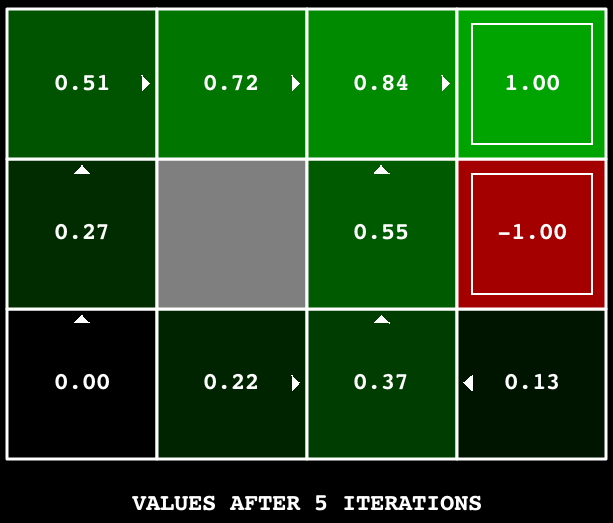
\includegraphics[width=0.5\textwidth]{2Grundlagen/33Policy.png}
\caption{Trainierte Policy nach 5 Iterationen. Jede Zelle zeigt den geschätzten Wert des Zustands und die von der Policy empfohlene Aktion. Grüne Zellen kennzeichnen positive Belohnungen, die rote Zelle kennzeichnet eine negative Belohnung.}
\label{fig:trained_policy}
  \cite{klein_abbeel_cs188}
\end{figure}
%
\paragraph{Pseudocode}
Die Aktualisierung der Policy-Parameter, wie in Gleichung \ref{eq:policy_gradient} beschrieben, erfolgt nach dem folgenden Schema:
\begin{algorithmic}
\STATE Initialisiere die Policy-Parameter \(\theta\)
\STATE Setze die Lernrate \(\alpha\)
\FOR{jede Episode}
    \STATE Initialisiere den Zustand \(s\)
    \WHILE{\(s\) kein terminaler Zustand ist}
        \STATE Wähle Aktion \(a\) basierend auf der aktuellen Policy \(\pi(s; \theta)\)
        \STATE Führe Aktion \(a\) aus, beobachte Belohnung \(r\) und neuen Zustand \(s'\)
        \STATE Aktualisiere die Policy-Parameter:
        \STATE \(\theta \leftarrow \theta + \alpha \nabla_{\theta} \log \pi(a | s; \theta) \cdot r\)
        \STATE \(s \leftarrow s'\)  \# Wechsel zum neuen Zustand
    \ENDWHILE
\ENDFOR
\end{algorithmic}

\paragraph{Wahl der Aktion in Policy-Based-Methoden}

In Policy-Based Reinforcement Learning-Methoden erfolgt die Aktionsermittlung basierend auf einer Wahrscheinlichkeitsverteilung der aktuellen Policy \(\pi(s; \theta)\), oft repräsentiert durch die Softmax-Funktion ,\ref{fig:softmax} wie in Abbildung \ref{eq:softmax} illustriert \cite{russell2021ai}. Besonders effektiv sind diese Methoden in komplexen Umgebungen, wo lineare oder einfache Beziehungen zwischen Zuständen, Aktionen und Belohnungen fehlen \cite{SuttonBarto2018}. Die direkte Optimierung der Policy ohne separate Value-Funktion bietet Vorteile, stellt jedoch eine Herausforderung dar, da eine umfangreiche Erkundung des Zustandsraums für die Konvergenz notwendig ist \cite{morales2020grokking}. Ein häufiger Ansatz zur Aktionsermittlung in diskreten Räumen ist der Epsilon-Greedy-Algorithmus \ref{eq:epsilon_greedy}, der die Balance zwischen Exploration und Exploitation hält \cite{SuttonBarto2018}.

\paragraph{Einschränkungen von Policy-Based-Methoden}
%
Policy-Based Methoden im Reinforcement Learning, effektiv in diskreten und kontinuierlichen Aktionsräumen, stoßen in komplexen Umgebungen an Grenzen. Ihre Hauptherausforderung ist die benötigte umfangreiche Erkundung des Zustandsraums für die Konvergenz, was in kostspieligen oder riskanten Szenarien praktisch problematisch sein kann \cite{SuttonBarto2018}. Zudem konvergieren sie langsamer als Value-Based-Methoden, besonders in Umgebungen mit vielen Zuständen oder hoher Dimensionalität, da die direkte Optimierung der Policy ohne konkrete Werteschätzungen aufwendiger ist \cite{SuttonBarto2018}. Diese Methoden sind zwar theoretisch für kontinuierliche Aktionsräume geeignet, ihre Effektivität kann jedoch in der Praxis durch feingranulare Aktionen und schwer abschätzbare Konsequenzen begrenzt sein.
